\begin{figure}[H]
\centering
\begin{minipage}{0.49\textwidth}
\centering
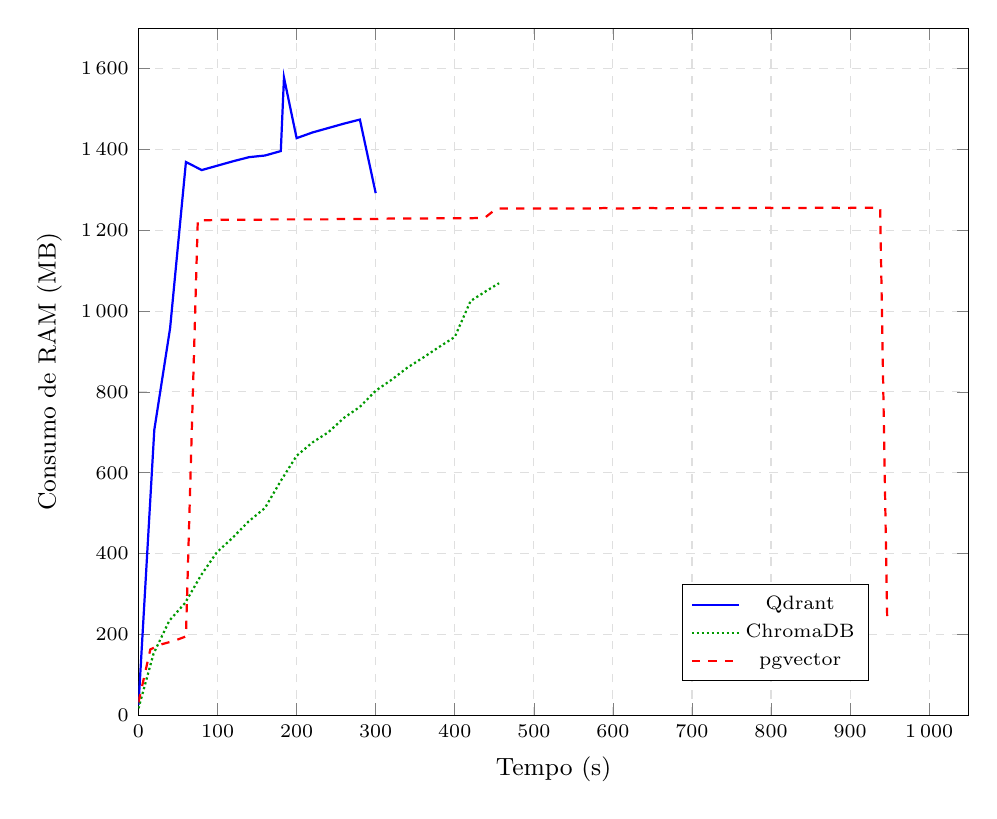
\begin{tikzpicture}
\begin{axis}[
    width=\textwidth, height=0.85\textwidth,
    xlabel={Tempo (s)}, ylabel={Consumo de RAM (MB)},
    xmin=0, xmax=1050, ymin=0, ymax=1700,
    /pgf/number format/1000 sep={\,},
    grid=major, grid style={dashed, gray!25},
    legend style={at={(0.88,0.05)}, anchor=south east, font=\scriptsize},
    tick label style={font=\scriptsize}, label style={font=\small}
]
\addplot[color=blue, solid, thick, mark=none] coordinates {
    (0,25) (20,706) (40,958) (60,1369) (80,1349) (100,1360) (120,1371) (140,1381) (160,1385) (180,1396) (184,1578) (200,1428) (220,1442) (240,1453) (260,1464) (280,1474) (300,1292)
};
\addlegendentry{Qdrant}
\addplot[color=green!60!black, densely dotted, thick, mark=none] coordinates {
    (0,17) (19,152) (39,234) (59,278) (79,346) (99,403) (119,439) (139,479) (160,513) (180,580) (200,642) (220,675) (240,700) (260,736) (280,763) (300,803) (320,830) (340,860) (360,885) (380,911) (400,936) (420,1025) (440,1050) (456,1069)
};
\addlegendentry{ChromaDB}
\addplot[color=red, dashed, thick, mark=none] coordinates {
    (0,32) (15,163) (30,176) (45,184) (60,195) (75,1225) (90,1225) (105,1226) (120,1226) (135,1226) (151,1226) (166,1227) (181,1227) (196,1227) (211,1227) (226,1227) (241,1227) (256,1228) (272,1228) (287,1228) (302,1228) (317,1229) (332,1229) (347,1229) (362,1229) (377,1230) (393,1230) (408,1230) (423,1230) (438,1231) (453,1254) (468,1254) (483,1254) (499,1254) (514,1254) (529,1254) (544,1254) (559,1254) (574,1254) (589,1255) (605,1254) (620,1254) (635,1255) (650,1255) (665,1254) (680,1255) (695,1255) (711,1255) (726,1255) (741,1255) (756,1255) (771,1255) (786,1255) (798,1256) (801,1255) (817,1255) (832,1255) (847,1255) (862,1256) (877,1256) (892,1255) (908,1256) (923,1256) (938,1255) (947,229)
};
\addlegendentry{pgvector}
\end{axis}
\end{tikzpicture}
\caption*{(a) Métrica L2}
\end{minipage}%
\hfill
\begin{minipage}{0.49\textwidth}
\centering
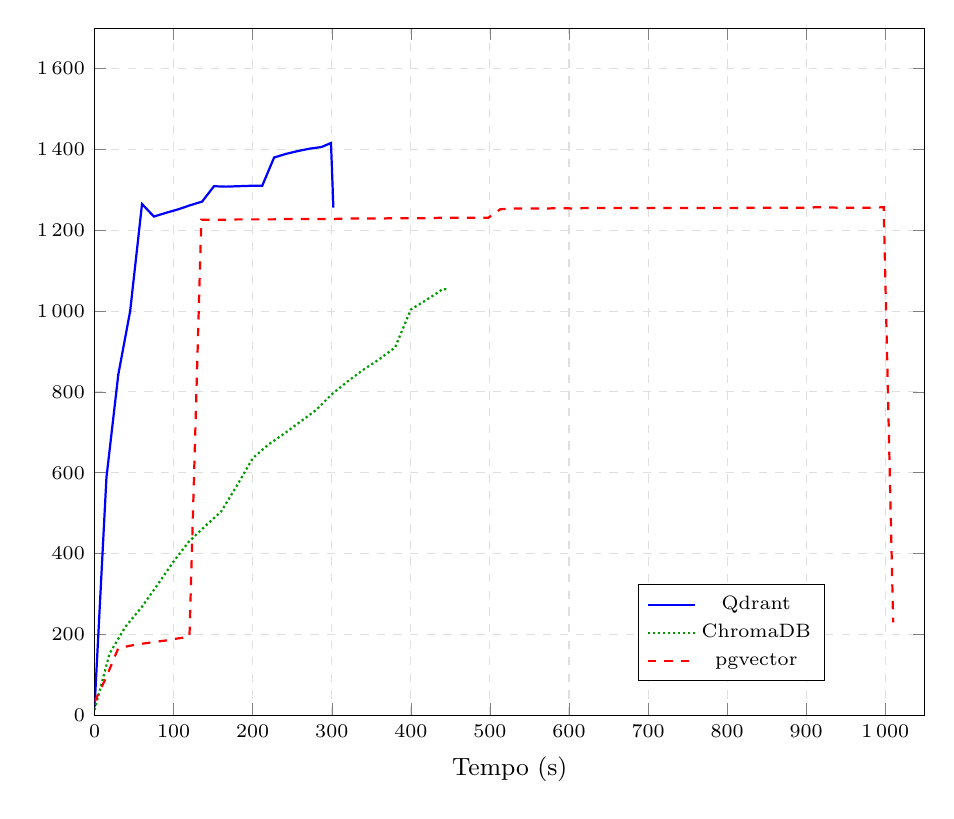
\begin{tikzpicture}
\begin{axis}[
    width=\textwidth, height=0.85\textwidth,
    xlabel={Tempo (s)}, ylabel={},
    xmin=0, xmax=1050, ymin=0, ymax=1700,
    /pgf/number format/1000 sep={\,},
    grid=major, grid style={dashed, gray!25},
    legend style={at={(0.88,0.05)}, anchor=south east, font=\scriptsize},
    tick label style={font=\scriptsize}, label style={font=\small}
]
\addplot[color=blue, solid, thick, mark=none] coordinates {
    (0,20) (15,588) (30,843) (45,1000) (60,1265) (75,1234) (90,1243) (106,1252) (121,1262) (136,1271) (151,1309) (166,1308) (181,1309) (196,1310) (212,1310) (227,1380) (242,1389) (257,1396) (272,1402) (287,1406) (299,1416) (302,1256)
};
\addlegendentry{Qdrant}
\addplot[color=green!60!black, densely dotted, thick, mark=none] coordinates {
    (0,13) (19,153) (39,219) (59,266) (79,321) (99,378) (119,429) (140,468) (160,504) (180,568) (200,636) (220,670) (240,697) (260,726) (280,755) (300,794) (320,826) (340,855) (360,881) (380,910) (400,1004) (420,1028) (440,1054) (445,1054)
};
\addlegendentry{ChromaDB}
\addplot[color=red, dashed, thick, mark=none] coordinates {
    (0,33) (15,95) (30,166) (45,172) (60,177) (75,181) (90,185) (105,190) (120,194) (135,1226) (151,1226) (166,1226) (181,1227) (196,1227) (211,1227) (226,1227) (241,1228) (256,1228) (272,1228) (287,1228) (302,1228) (317,1229) (332,1229) (347,1229) (362,1229) (377,1230) (392,1230) (408,1230) (423,1230) (438,1231) (453,1231) (468,1231) (483,1231) (498,1231) (513,1252) (529,1254) (544,1254) (559,1254) (574,1254) (589,1255) (604,1254) (620,1255) (635,1255) (650,1255) (665,1255) (680,1255) (695,1255) (710,1255) (726,1255) (741,1255) (756,1255) (771,1255) (786,1255) (801,1255) (816,1255) (832,1256) (847,1256) (862,1256) (877,1256) (892,1256) (907,1255) (910,1257) (923,1257) (938,1256) (953,1256) (968,1256) (983,1256) (998,1257) (1010,230)
};
\addlegendentry{pgvector}
\end{axis}
\end{tikzpicture}
\caption*{(b) Similaridade de Cosseno}
\end{minipage}
\caption{Evolução do consumo de RAM de cada contentor durante a inserção de 1\,000\,000 de vetores e a construção do índice HNSW. Cada série começa com o contentor acabado de reiniciar e termina quando o índice está construído. Valores absolutos medidos pelo \texttt{docker stats}.}
\label{fig:profiling_memoria}
\end{figure}
